\section{Architecture Overview}
\label{section:architecture}

\begin{wrapfigure}{r}{0.36\textwidth}
    \centering
    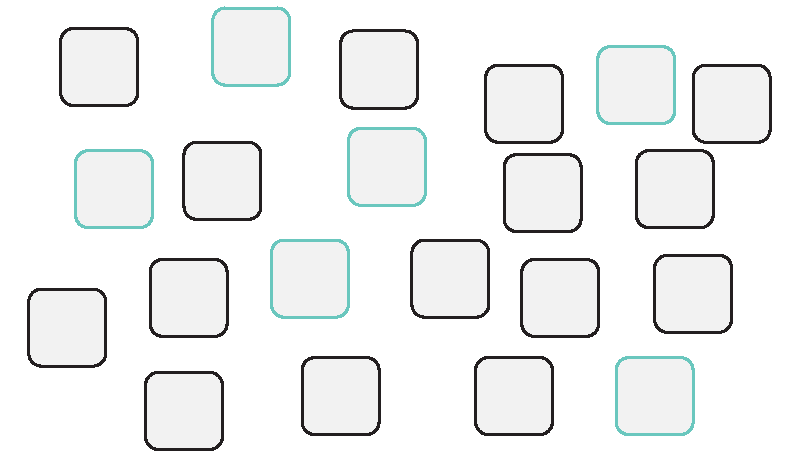
\includegraphics[width=0.35\textwidth]{img/cohort.pdf}
    \caption{A single team (in teal), randomly selected from a group of nodes.}
    \label{fig:team}
\end{wrapfigure}

In order to protect a user's digital sovereignty, the \name protocol utilizes accelerated mix networks to ensure confidentiality. A mix network~\cite{mix_81} is a routing protocol that uses cryptography to dissociate the origin, contents, and destination of a message. A ``message'' in this context could be simply a text message, or else a payment transaction on a blockchain. The \name protocol uses mix networks in combination with a distributed ledger to create a confidential blockchain. 

Unlike other blockchain protocols, in the \name protocol, groups of nodes are deterministically organized into teams. \name teams are temporary, and exist only for the duration of the block they are responsible for generating. The team uses a consensus protocol, explained in Section~\ref{section:consensus}, to validate and authenticate operations that anonymize each encrypted message, independently agree to process all messages before decryption, and then independently decrypt~\footnote{Messages are still end-to-end encrypted over the network.} and process each message. Following block generation, the team disbands and member nodes become available to be placed on a new random team. As shown in Figure~\ref{figure:simple-architecture}, the team allows messages to be sent both directions with anonymity. 

\begin{wrapfigure}{L}{0.58\textwidth}
    \centering
    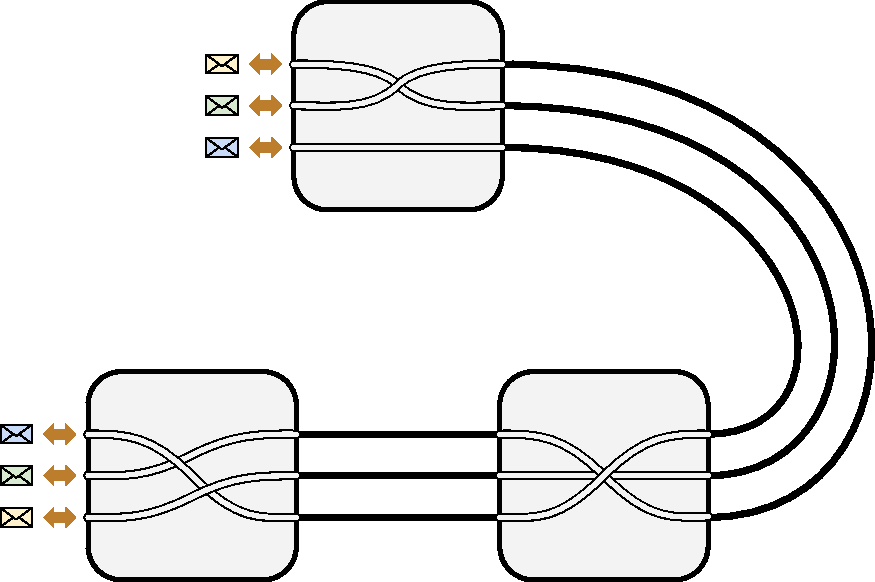
\includegraphics[width=0.5\textwidth]{img/Simple-Architecture.pdf}
    \caption{Each team creates an anonymous, verifiable, bi-directional transaction channel to process each block in the blockchain.}
    \label{figure:simple-architecture}
\end{wrapfigure}

All operations conducted by \name teams are accelerated through the use of precomputation~\cite{precomps}. These precomputations produce a template that dictates how the nodes within a team must process information during block generation. Consequently, the template is completely defined before any message information arrives for block generation. The use of precomputation ensures confidentiality while dramatically increasing the speed at which information can be processed to generate a block.

Nodes must be elected to participate in processing the messages and transactions on the \name network. In order to be eligible for election, a node is required to stake tokens on the network. Once elected, a node is eligible to be placed into an \name team. 

\begin{figure}[H]
    \centering
    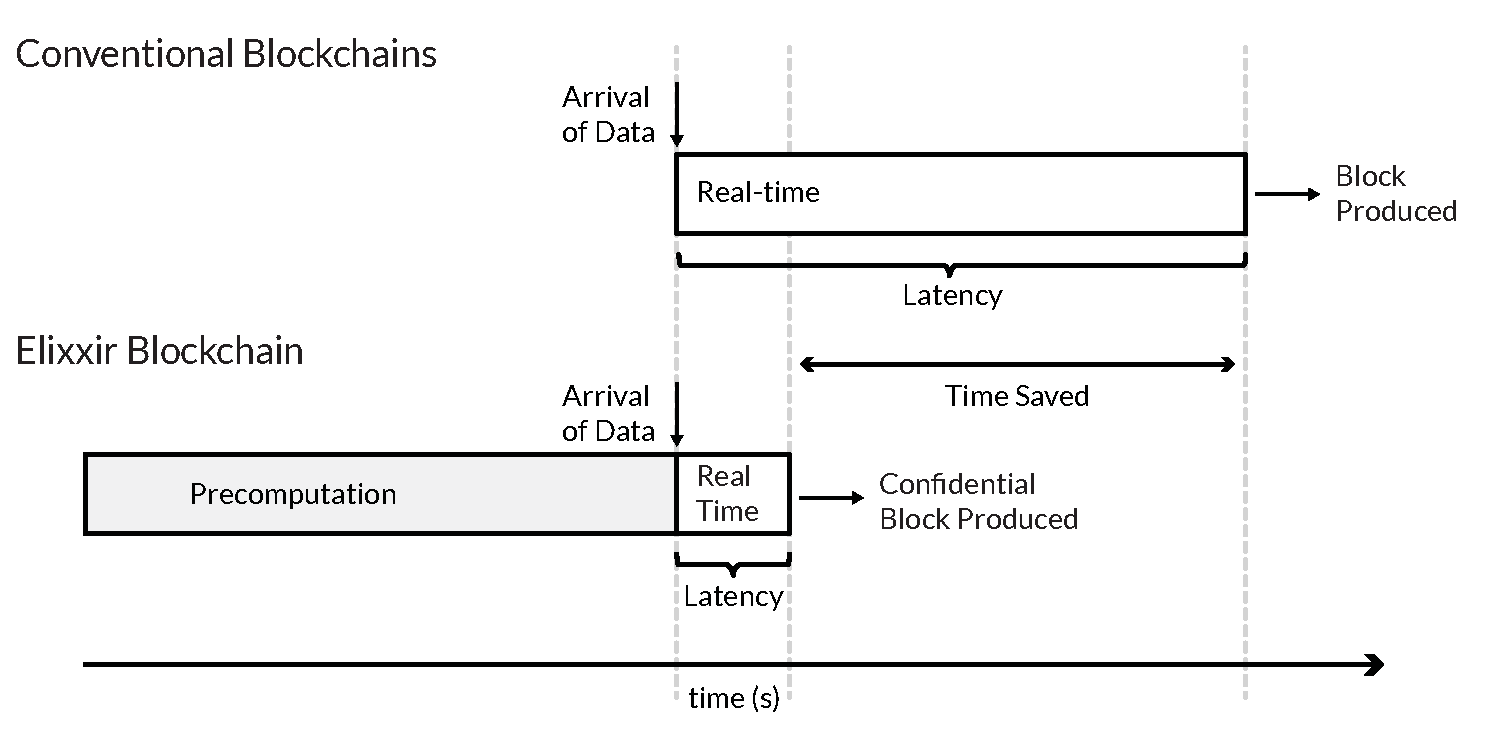
\includegraphics[width=\textwidth]{img/Processing.pdf}
    \caption{Time-consuming, computationally-intensive team precomputation is performed before transactions are sent or received. This allows very fast real-time computation of transactions to generate each block in the blockchain. The use of precomputation decouples security from latency as seen in conventional blockchains, delivering a greater level of security without the latency penalty.}
    \label{figure:processing}
\end{figure}

There are two phases involved in block production by an \name team as depicted in Figure~\ref{figure:processing}. First, the team performs a computationally-intensive precomputation as discussed above, producing a unique template defining how the information or messages of the block will be processed. When messages arrive, the nodes of the team work together to process the messages in real time according to this unique template, a process that takes less than 1/20th of the precomputation time. 

Unlike sharding proposals or the lightning network~\cite{lightning}, \name teams cannot influence the consensus mechanism's integrity as all aspects of block production are independently predetermined in a strict, verifiable, and immutable manner. Additionally, all nodes in a team independently provide proofs that validate the block prior to final block confirmation. 

To ensure proper system functionality, nodes collectively and independently generate cryptographic proofs as commits of batch integrity prior to decryption. In the event that commits do not match, all proofs produced by the nodes can be inspected to identify node failure or malfeasance. Once a malicious or malfunctioning node has been identified, honest nodes refuse further contact and broadcast proof of malfeasance or malfunction to the rest of the network. If a node is verified to be malicious, it loses its stake of tokens, which are burned, and the node is ejected from the network.  These, and additional security mechanisms, allow users to prove incorrect handling of their transaction, while rendering them unable to accuse the nodes or the team falsely.

\subsection{Scaling Strategy}

At any given time, tens to hundreds of teams will exist within the network in varying stages of precomputation. However, at any given time, only one team will be producing a block. These precomputations overlap in a cascade, as shown in Figure~\ref{figure:processing-cascade}. Consequently, the throughput of the network increases with the addition of more nodes to the network forming more teams. This allows the platform to linearly scale its capacity with the addition of more nodes.

\begin{figure}[H]
    \centering
    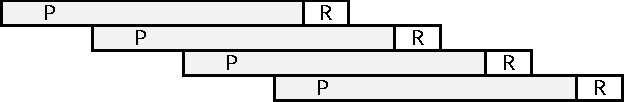
\includegraphics[width=\textwidth]{img/Processing-Cascade.pdf}
    \caption{Teams are organized into a cascade pipeline to maximize the number of transactions that can be processed by our platform.}
    \label{figure:processing-cascade}
\end{figure}

Increasing the number of teams results in increased network resilience as more teams must be brought down to impair or completely disrupt the network. As longer precomputation times become feasible, the number of messages processed by each team can also be increased. 

\subsection{Block Propagation}

Once generated, block data is broadcast to each node in the next team. Once the next active team has received the block data, data is then broadcast to the rest of the nodes in the network. This sequence prioritizes communication to the next team responsible for block generation, ensuring efficient block propagation.
